\section{Prepositional Phrase Attachment}
Machine reading and information extraction (IE)  projects have produced large resources with many millions of  facts  \cite{MitchellCHTBCMG15,suchanek2007yago}.  This wealth of knowledge  creates  a positive feedback loop for automatic knowledge base construction efforts: the accumulated knowledge can be leveraged to improve   machine reading; in turn,  improved  reading methods can be used to better  extract knowledge expressed using complex and  potentially ambiguous language.
 For example,  prepositional phrases (PPs)   express crucial information that  IE methods need to extract.
 % comprehensively extract facts. 
 However, PPs are a major source of  syntactic  ambiguity. In this paper, we propose to use semantic knowledge to  improve PP attachment disambiguation. 
 PPs such as  ``in", ``at", and ``for" express details about the  \textit{where, when,} and \textit{why}  of  relations and events. PPs   also state  attributes of nouns. 
 
     
         \begin{figure}[t]
         %
         \centering
         %
         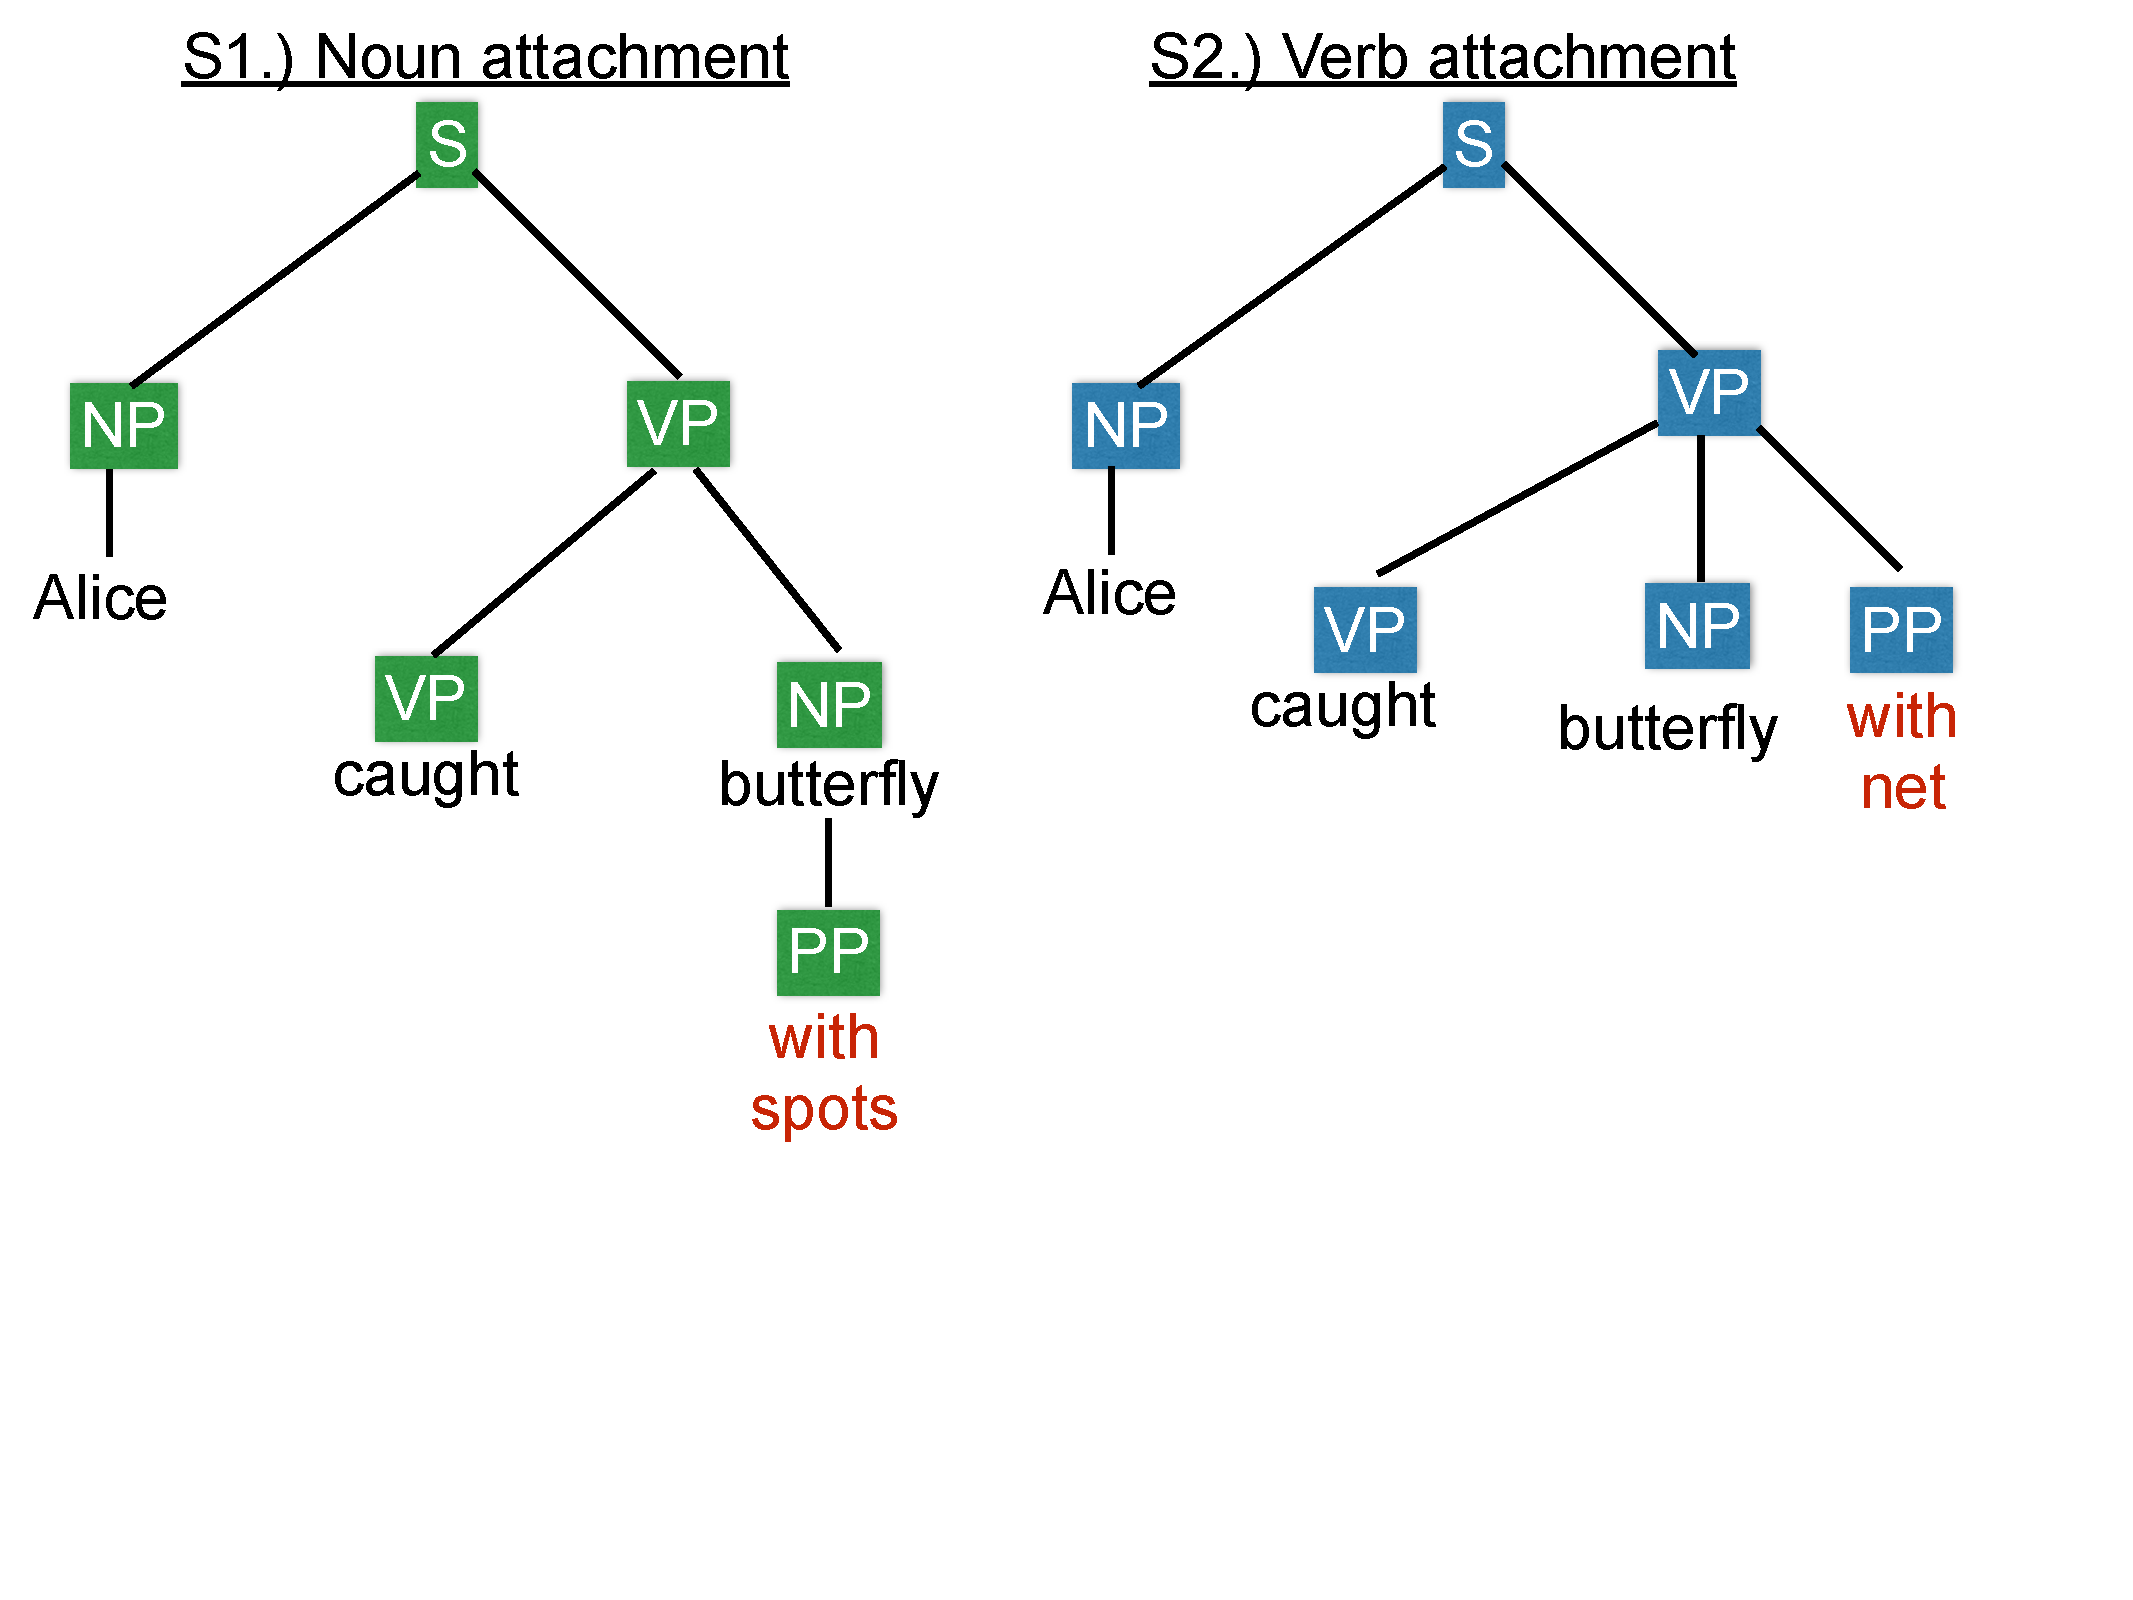
\includegraphics[width=1\columnwidth] {trees2.pdf}
         %\includegraphics[width=0.8\columnwidth] {results_objective_truth.jpg}
         %\includegraphics{images/pearl/entitytyes_precision04.png}
         %
         \vspace*{-2.6cm}
         \caption{Parse trees where the prepositional phrase (PP) attaches to the noun, and to the verb.}
         % The only difference in the parse trees are the PP attachment sites, resulting in trees of different structures.}
         % and hence the sentence structures are different. } 
         %
         \label{fig:deptrees}
         %
         \end{figure}

                     \begin{table}[h]
                              \centering
                              \small{
                                       \begin{tabular}{|p{1.8cm}|p{4.9cm}|}
                                         % \hline
                                       %&  {\bf Definition \& Example(s)}  \\
                                         \hline
                                        % \newline -receive(agent, patient, source) \\
                                         % \newline -isA(tea,beverage)\\
                                         Relations &  Noun-Noun binary relations  \newline \textit{ (Paris, located in, France)} \newline \textit{(net, caught, butterfly)}\\
                                         \hline
                                         Nouns &  Noun semantic categories \newline \textit{(butterfly, isA, animal)}  \\
                                         \hline
                                         Verbs & Verb roles \newline  \textit{caught(agent, patient, instrument)} \\
                                         \hline
                                         % \newline -(fork, used for, eating) \\
                                         Prepositions& Preposition  definitions \newline  
                                         \textit{ f(for)= used for, has purpose, ...}  
                                         \newline \textit{f(with)= has, contains, ...}  \\
                                         \hline
                                         Discourse &  Context \newline  $n0 \in \{n0, v, n1, p, n2\}$\\
                                         \hline
                                       \end{tabular}
                                       \caption{Types of background   
                                       knowledge used in this paper to determine PP attachment.}
                                         \label{tab:knowledge}
                                         }      
                                       \end{table}     
        
 
 As an example, consider the following sentences: \textit{ S1.) Alice caught the butterfly with the spots. S2.) Alice caught the butterfly with the net. }  S1 and S2 are syntactically different, this is evident from their corresponding parse trees in Figure \ref{fig:deptrees}. Specifically,  S1 and S2  differ in where their PPs attach. In  S1,  the butterfly has spots and therefore  the PP, ``with the spots'', attaches to the \textit{noun}. For relation extraction, we  obtain a \textit{binary} relation of the form:  
 $\langle$Alice$\rangle$  caught $\langle$butterfly with  spots$\rangle$.
However, in S2, the net is the instrument used for catching and therefore  the PP,  ``with the net", attaches to the \textit{verb}.  For relation extraction, we get a \textit{ternary} extraction of the form:
%\begin{itemize}
%\item[]
 $\langle$Alice$\rangle$  caught $\langle$butterfly$\rangle$ with $\langle$net$\rangle$.
%\item[] $\langle$The government$\rangle$  discovered $\langle$irregularities$\rangle$ in $\langle$June$\rangle$
%\end{itemize
 
The PP attachment problem is often defined as follows: given a PP occurring within a  sentence where there are multiple possible attachment sites for the PP, choose the most plausible attachment site. 
%Notice that in the examples we have given so far, there were only two possible attachment sites, the noun and the verb.
% as shown in Figure \ref{fig:deptrees} with a parse tree corresponding to each type.
 In the literature,  prior work going as far back as \cite{BrillR94,Ratnaparkhi1994,Collins95} has  focused on the  language pattern that causes most PP ambiguities, which is the  4-word sequence: $\{v, n1, p, n2\}$ (e.g., $\{${\em caught, butterfly, with, spots}$\}$). The task is  to   determine if  the prepositional phrase $(p,n2)$  attaches to  the verb $v$ or to the first noun $n1$.
Following common practice,  we focus on  PPs occurring as $\{v,n1,p,n2\}$ quadruples ---  we shall refer to these as  \textit{PP quads}. 

The approach we present here differs from prior work in two main ways. First, we make extensive use of semantic knowledge about nouns, verbs, prepositions, pairs of nouns, and  the discourse context in which a PP quad occurs. Table \ref{tab:knowledge}  summarizes the types of  knowledge we considered in our work. Second, in training our model, we rely on both labeled and unlabeled data, employing an expectation maximization (EM) algorithm \cite{Dempster77maximumlikelihood}. 


         \begin{figure}[t]
                 %
                 \centering
                 %
                 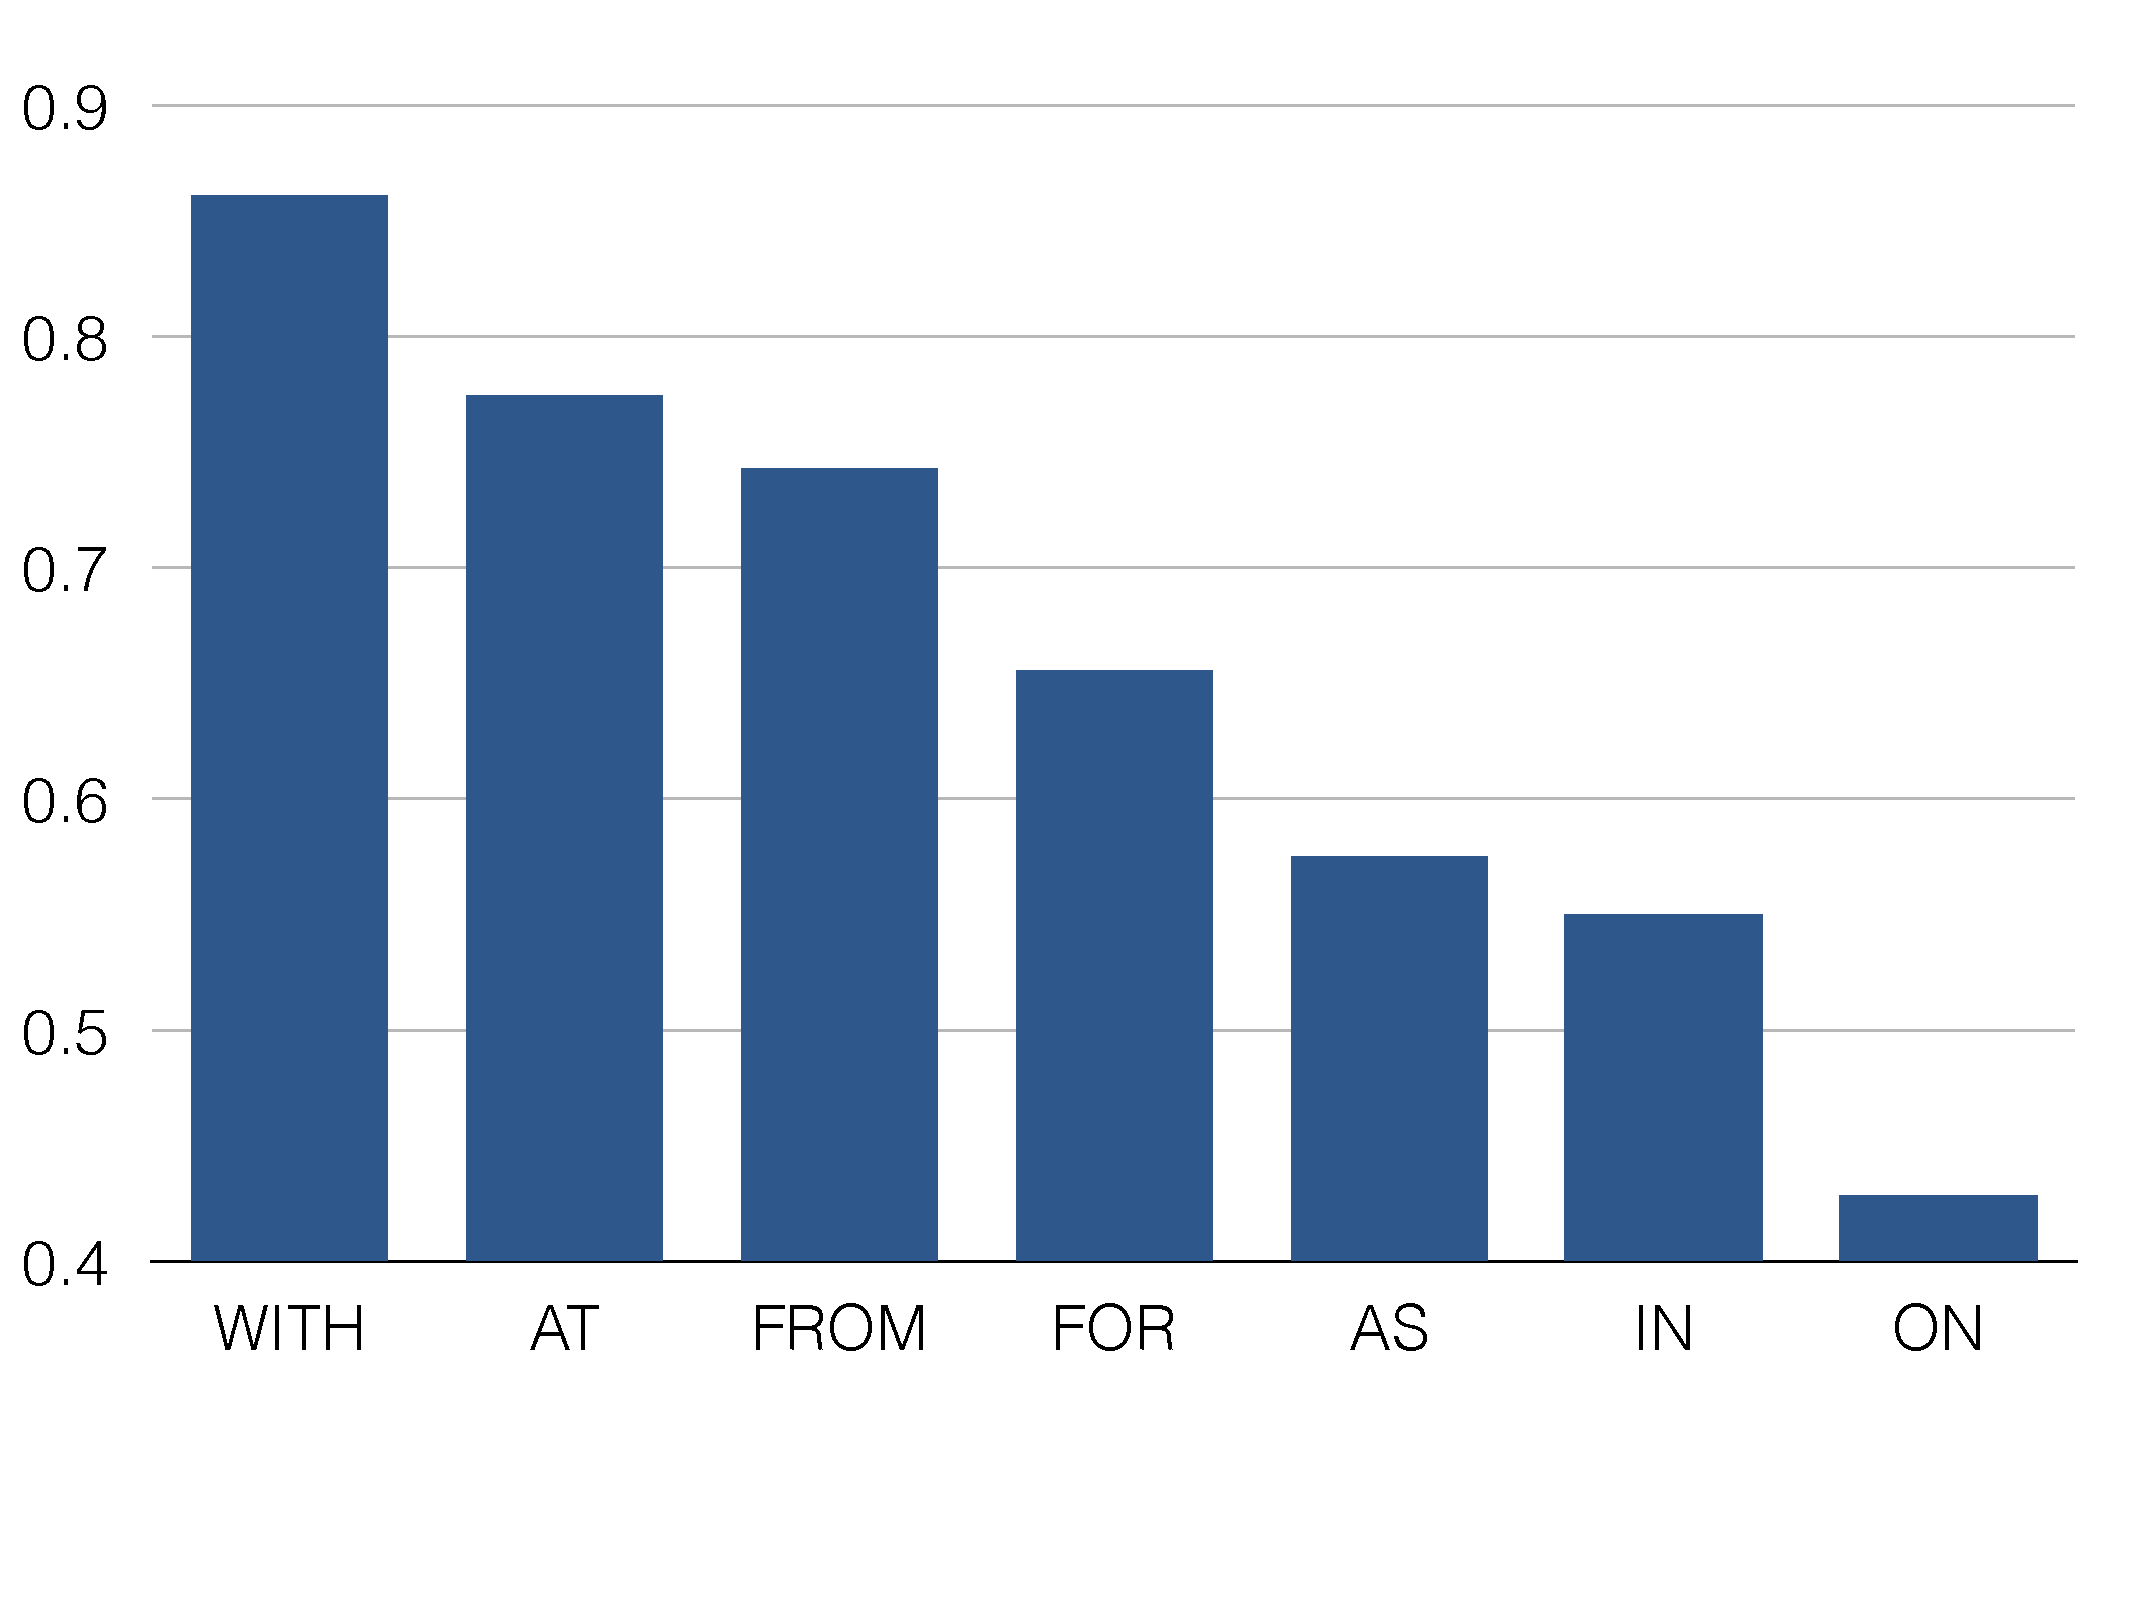
\includegraphics[width=0.80\columnwidth] {mainresults-0.pdf}
                 \vspace*{-0.8cm}
                 \caption{Dependency parser PP attachment accuracy for various frequent prepositions.}
                 % The only difference in the parse trees are the PP attachment sites, resulting in trees of different structures.}
                 % and hence the sentence structures are different. } 
                 %
                 \label{fig:parser}
                 %
                 \end{figure}  
        
                
\paragraph{Contributions}
In summary,  our main contributions are: 
 
\textit{1)~Semantic Knowledge:} 
Previous  methods largely rely on  corpus statistics. Our approach  draws upon 
 diverse sources of background knowledge, leading to performance improvements.
 
\textit{2)~Unlabeled  Data:} In addition to training on labeled  data, we also make use of a large amount of unlabeled data. This enhances our method's ability to generalize to diverse data sets. 
% in settings with incomplete data. 
%Our experiments show that  unlabeled data helps performance over diverse test collections by introducing new  features not in the labeled data.

\textit{3)~ Datasets:} In addition to the standard Wall Street Journal corpus (WSJ)~\cite{Ratnaparkhi1994}, we labeled two new datasets for testing purposes, one from Wikipedia (WKP), and another from the  New York Times Corpus (NYTC). We make  these datasets freely available for future research.  In addition, we have applied our  model to over 4 million 5-tuples of the form $\{n0, v, n1, p, n2\}$, and we also make this dataset  available\footnote{http://rtw.ml.cmu.edu/resources/ppa} for research into ternary relation extraction beyond spatial and  temporal scoping.